\documentclass{article}
\usepackage{NIPS10,times}
%\documentstyle[nips07submit_09,times]{article}
\usepackage[square,numbers]{natbib}
\usepackage{amsmath, epsfig}
\usepackage{amsfonts}
\usepackage{subfigure}
\usepackage{graphicx}
\usepackage{amsfonts}
\usepackage{algorithm}
\usepackage{algorithmic}
\usepackage{easybmat}
\usepackage{listings}
\usepackage{footmisc}
\renewcommand\algorithmiccomment[1]{// \textit{#1}}
%
\newcommand{\ignore}[1]{}
\newcommand{\comment}[1]{}
\DeclareMathOperator*{\argmax}{arg\,max}

% decrease spacing in itemize
\newenvironment{itemize*}{
\begin{itemize}
  \setlength{\itemsep}{0.7em}
  \setlength{\parskip}{0pt}
  \setlength{\parsep}{0pt}
}{\end{itemize}}

\title{Introduction to Data Science\\Homework Assignment 3}

\author{
Michael Discenza\\\\
Columbia University, New York, NY 10027, USA \\
\texttt{mad2200@columbia.edu}
}
}

% The \author macro works with any number of authors. There are two commands
% used to separate the names and addresses of multiple authors: \And and \AND.
%
% Using \And between authors leaves it to \LaTeX{} to determine where to break
% the lines. Using \AND forces a linebreak at that point. So, if \LaTeX{}
% puts 3 of 4 authors names on the first line, and the last on the second
% line, try using \AND instead of \And before the third author name.

\newcommand{\fix}{\marginpar{FIX}}
\newcommand{\new}{\marginpar{NEW}}
\newcommand{\X}{\mathcal{X}}

\nipsfinalcopy

\begin{document}

\maketitle



%%%%%%%%%%%%%%%%%%%%%%%%%%%%%%%%%%%%%%%%%%%%%%%%%%%%%%%%%%%%%%%%%%%%%%%%%%%%%%%%%%%%%%%%%%
%%%%%%%%%%%%%%%%%%%%%%%%%%%%%%%%%%%%%%%%%%%%%%%%%%%%%%%%%%%%%%%%%%%%%%%%%%%%%%%%%%%%%%%%%%
%%%%%%%%%%%%%%%%%%%%%%%%%%%%%%%%%%%%%%%%%%%%%%%%%%%%%%%%%%%%%%%%%%%%%%%%%%%%%%%%%%%%%%%%%%

\section{FlowingData.com Visualization Tutorial}

I went through the following tutorials on FlowingData:
\begin{itemize}\itemsep1pt \parskip0pt \parsep0pt
  \item More on Making Heat Maps in R 
  \item How to Visualize and Compare Distributions
  \item How to Make Bubble Charts
\end{itemize}
For my graph, I tried to use Nathan's tutorial on bubble charts to visualize data about the gender pay gap from the Bureau of Labor Statistics.  

The graphs that I wanted to combine and the data from which the graphs were made are found here:
http://www.bls.gov/opub/ted/2009/ted\_20090807.htm

% latex table generated in R 2.15.1 by xtable 1.7-0 package
% Wed Oct 24 12:54:06 2012
\begin{table}[H]
\begin{center}
\begin{tabular}{rlrrrr}
  \hline
 & Occupational Group & Women & W Earnings & Men & M earnings \\ 
  \hline
1 & Management  & 4535000 & 979 & 6687000 & 1384 \\ 
  2 & Business and financial operations  & 2928000 & 885 & 2159000 & 1167 \\ 
  3 & Computer and mathematical  & 828000 & 1088 & 2516000 & 1320 \\ 
  4 & Architecture and engineering  & 334000 & 1001 & 2319000 & 1286 \\ 
  5 & Life, physical, and social science  & 477000 & 931 & 603000 & 1156 \\ 
  6 & Community and social services  & 1117000 & 753 & 791000 & 860 \\ 
  7 & Legal & 693000 & 962 & 506000 & 1696 \\ 
  8 & Education, training, library  & 4883000 & 818 & 1794000 & 1020 \\ 
  9 & Arts, design, entertainment, sports & 689000 & 777 & 882000 & 951 \\ 
  10 & Healthcare practitioner & 4052000 & 909 & 1362000 & 1210 \\ 
   \hline
\end{tabular}
\end{center}
\end{table}

\begin{figure}[H]
\begin{center}
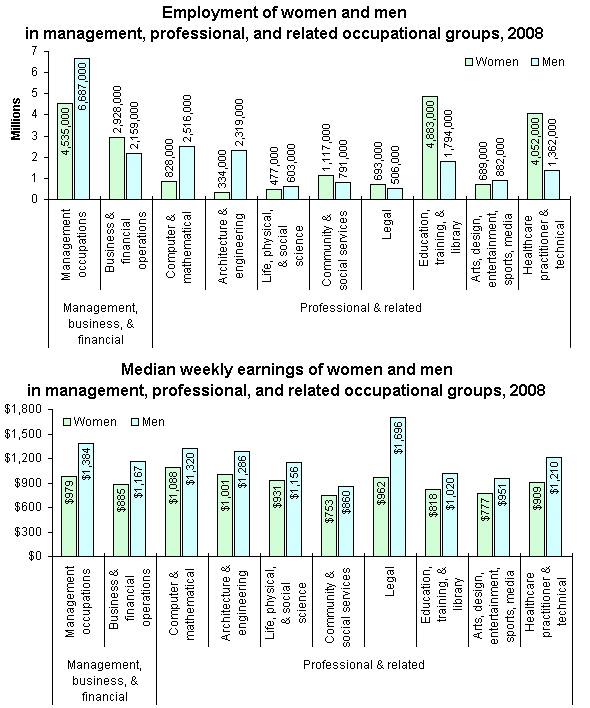
\includegraphics[width=1\columnwidth]{bls_graph.jpg}
\caption{These are the two graphs that the BLS uses to illustrate the gender pay gap by occupation.}
\end{center}
\end{figure}



\begin{figure}[H]
\begin{center}
\includegraphics[width=1\columnwidth]{gender_old.eps}
\caption{This is the graph that I made using the methods that Nathan used in his tutorial.  I was not able to to make sure the coordinates were square to accurately show the slope of the line and indicate the pay inequality between men and women nor show the additional dimension of percentage women in each occupation group with a color scale.}
\end{center}
\end{figure}

\begin{figure}[H]
\begin{center}
\includegraphics[width=1\columnwidth]{gender.eps}
\caption{As an alternative to the symbols() graphing function that Nathan used, I recreated the graph using Hadley Wickham's ggplot2 package.  The graph shows all of the information that I wanted it to show, but I think the end product might not be the most ideal because it contains perhaps too much information for a viewer to easily interpret and the labels associated with the data points are not aesthetically pleasing.  This is something that I might have been able to change by editing them in Inkscape and drawing arrows from the labels to their respective data points in order to reduce the clutter on the plot.}
\end{center}
\end{figure}

It was very easy to follow Nathan's tutorials and helpful that he had explained what certain options do.  In general, I spend hours, like multiple hours trying to get graphs to look the way I want becasue there aren't good cheat sheets and there isn't good graphical documentation for packages like ggplot.  Next I would like to find or make a cheat sheet so that I don't spend as much time on visualizing data as I have been.

\section{The Data Science of Art}

I think that the points that everyone brings up about using social network analysis with data from service like Foursquare and Instagram are quite valid.  And certainly I would say that the list of metrics to measure that Anderson created is quite exhaustive.  I think though that Anderson’s list and mentality is honestly more like the U.S. News \& World Report's rankings of Universities and Hospitals.  Though it’s unclear whether museums would pay any attention to their rankings or if those rankings would even be published or circulated, but if they did start paying attention to their rank or composite index based on this data, we have to ask if that would be actually a good thing for the museums in terms of satisfying their more intrinsic goals or if it would lead to manipulation of metrics for higher rank like what happens in some colleges.  I also think that the index fails to account for the various different missions of museums.  For instance a Museum like the Brooklyn Museum, my favorite art Museum in the city, and one that gives me great joy has an altogether different character and atmosphere than the MoMA or the Met.  

Moreover the rankings would probably create a consolidation of donations and it would make the process by which benefactors might figure out how to “best spend” their money overly market-based.  Though I am not in a position to endow and collections or donate much more money than a suggested entry fee to a museum, I imagine that there is an importance that a donor have some kind of personal connection the museum, some more intimate reason for donating as to make the donation somehow more legitimate.  

Having articulated my discomfort with this idea of an index, I would like to focus now on some of the ways that I think methods in data science and machine learning might be useful for providing specific insights about user experience to help museum management enhance the enjoyment of their guests.  

First I think it is important that internally as opposed to externally museum management and boards devise a set of metrics and indicators that they find to be important for their particular priorities.  Once they do this they should maintain some kind of “dashboard” that is updated with at least some consistent frequency, as has become standard organizational practice so going forward, they can have sense of how various interventions they make in guest experiences effect the metrics that they deem important.

Second, I think that art museums (or maybe some new tech consulting firm that could specialize in art museums) should begin to leverage technology that has been used by retailers for a good amount of time now including motion tracking with web cams to better track guest interest in certain piece of certain kinds based on the among of time of the inferred position of units (the guests) within a map of the museum.  This would allow the museums to make a number of useful interventions including feeding information and feedback to curators, better planning operations and queuing strategies to avoid lines and waits (basically what Disney Operations Research people do).

Finally, museums should try to experiment with new service like Art.sy and develop (or use a template for some kind of mobile app) to create mobile apps to scan QR codes associated with pieces of art to read descriptions and facts about the works they are viewing on their smart phones.  These would be services presented under the auspices of providing enhanced information about works they are viewing, but that just as importantly for the museum management serve to create a rich click-stream-like dataset that can be cross referenced with the visual tracking of users and stored from one visit to the next to better understand how guests’ interaction with a museum’s collection (or multiple museums’ collections) varies over time.


\section{Finance; Time Series and Regression}
[Kaushik Reddy and I spent a few hours working together on the code and then split up for the remainder of the project due to schedule constraints]

\begin{figure}[H]
\begin{center}
\includegraphics[width=1\columnwidth]{IBM_log_return.eps}
\caption{}
\end{center}
\end{figure}


\begin{figure}[H]
\begin{center}
\includegraphics[width=1\columnwidth]{IBM_log_volume.eps}
\caption{}
\end{center}
\end{figure}


I fit a model by regressing log returns on the previous two days' returns (an autoregressive second order model).  This procedure was conducted by manually lagging the data and using the two previous days' log returns as perdictor vectors, not using the AR or ARIMA functions. I did fit an AR function that found the optimal number of predictors to be 36 using AIC as the selection criterion for the model, but was unable to use the model with R's predict function and such a model would likely have been tremendously overfit. 

In the second order autoregressive model, the log returns of the previous day proved to be significant.
% latex table generated in R 2.15.1 by xtable 1.7-0 package
% Mon Oct 22 09:45:38 2012
% latex table generated in R 2.15.1 by xtable 1.7-0 package
% Mon Oct 22 11:08:46 2012
\begin{table}[H]
\begin{center}
\begin{tabular}{rrrrr}
  \hline
 & Estimate & Std. Error & t value & Pr($>$$|$t$|$) \\ 
  \hline
(Intercept) & 0.0001 & 0.0004 & 0.26 & 0.7919 \\ 
  Predictor1 & -0.0502 & 0.0190 & -2.64 & 0.0083 \\ 
  Predictor2 & -0.0149 & 0.0190 & -0.79 & 0.4318 \\ 
   \hline
\end{tabular}
\end{center}
\end{table} 
Despite the significance of the coefficients fit by the model, the signal was week and often times not in the right direction of the log return.  Run over the course of two years (on totally new test data after the model was fit to the previous 10 years of training data), the model earned a log return of -0.2447558, meaning that with this model, one would actually lose money.

This resulting log return is however based on a number of simplifying assumptions: 1) there are zero transaction fees, 2)when the model predicts either a positive or a negative return correctly, it makes the full log return associated with that day regardless of whether it was on the positive or negative side [i.e., the options market for purchasing shorts is perfectly efficient], 3) the model was not updated over time- it was only fit to the training data and was not recalibrated to either forget previous data points over time or incorporate new data as time progressed.

\begin{figure}[H]
\begin{center}
\includegraphics[width=1\columnwidth]{performance.eps}
\caption{This graph shows the performance of the model over the last 50 days of tranding.  When the red prediction line and the black line for actual log return have the same sign, the trading strategy makes money, and when they have opposite sides, it loses money}
\end{center}
\end{figure}


\begin{figure}[H]
\begin{center}
\includegraphics[width=1\columnwidth]{pl.eps}
\caption{An ideal cumulative P\&L graph would show a steady growth in profits.  This model failed to produce a steady trajecotry or profitability}
\end{center}
\end{figure}


\section{Get Glue Case Study}

Note that to do this problem, I spent a ton of time figuring out how to use AWS's EC2 and run RStudio through the browser, which was pretty cool, but when I went to actually do the processing, the code that ran on my own machine did not run correctly on the server so I just ended up using the first 10,000 records of the dataset for the exercise and did the processing locally.

Answers to questions (albiet on only a subset of the data):
\begin{description}\itemsep1pt \parskip0pt \parsep0pt
  \item [What actions can a user take?] \hfill \\
   Liking, disliking, or commenting
  \item [Number of Unique Users?]\hfill \\
   740 (based on userID and not display name, because the latter is not unique)
  \item [Top 10 most popular movies?]\hfill \\
   "The Dark Knight", 
"Fight Club", "Pulp Fiction", "The Hangover", "Slumdog Millionaire", 
"Iron Man", "WALL-E", "Star Wars: Episode V: The Empire Strikes Back", 
"Indiana Jones and the Last Crusade", "Up", "Star Wars: Episode VI: Return of the Jedi"(based on the total number of likes each recieved)
  \item [Number of events that occured in 2011?]  \hfill \\
  I have no way of knowing only using this subset of the data
\end{description}
\hfill \\
\hfill \\
Other interesting questions that I proposed:
\begin{description}
  \item [Which user generates the most useful comments?] \hfill \\
  In the 10,000 record sample, there were not that many comments and even fewer comments marked as useful, only 5 actually.  But they were from the users with user IDs dandhroberts, kenjamd, PrinceAL, DelayedReality, and aka\_sulley (We could potentially design this piece of information back into the system and highlight his or her comments so that the other users could benefit the most)
  \item [Do more people rate movies or TV shows?] \hfill \\
  646 of the 740 users rated movies, but only 249 of those 740 users rated TV shows.  Another way of interpeting the question is that 469 users have rated only movies and no TV shows and only 72 people have rated TV shows and no movies.
  \item [Are the majority of the comments negative or positive?] \hfill \\
  To solve this, we could read the comments, but if we had a much larger data set that had more than 84 comments, that would be unfeasible, so we can assume that if the same user likes and makes a comment. [I actually struggled a lot getting this from the data-I think that I was trying to do this in a way that relied too much on primative operations and not plyr or reshape--I'll come to office hrs and maybe you can help me figure this out]
  \item [Genres?] \hfill \\
  Another interesting way to look at the data is to use the genres associated with the movies - very possible to get by scraping IMDB or using one of the various APIs that provides movie genres and figure out the distribution of likes of our users.  I did not have enough time to do this, but this is certainly something that would be useful to do.
  \item [Is there a correlation between the number of movies and number of TV shows a user rates/comments one? See graph below:]
\end{description}
\begin{figure}[H]
\begin{center}
\includegraphics[width=1\columnwidth]{getglue2.eps}
\caption{This plot shows the non-outlying counts of ratings and comments from users who have rated more than one title in each category. There seems to be a postive correlation bewteen the number of movies and the number of shows that users rate. Though this is supposed to be exploratory data analysis, I displayed the regression line that was fit using a first order linear model (which was found to have an R-squared value of 0.5949) for reference.  With this concentration of data near the origin and and only a few throughout the range, this is certainly a data set that does not meet the constant variance assumption for applying linear regression.  In order to apply a model to this kind of data, we need more users who might meet a minimum threshold of ratings, i.e. power users whose rate of Movie to TV show ratings we might actually be able to model}
\end{center}
\end{figure}



\section{Code Appendix}
All code (in easier to read form) as well as additional graphics files can be found on this assignment's git repository:
https://github.com/mdiscenza/Data-Science-HW3

\lstinputlisting[language=R]{hw3_visualization.R}
\lstinputlisting[language=R]{hw3_problem3_test_returns.R}
\lstinputlisting[language=R]{hw3_problem3_test-train_split.R}
\lstinputlisting[language=R]{hw3_problem4_try2.R}



%%%%%%%%%%%%%%%%%%%%%%%%%%%%%%%%%%%%%%%%%%%%%%%%%%%%%%%%%%%%%%%%%%%%%%%%%%%%%%%%%%%%%%%%%%
%%%%%%%%%%%%%%%%%%%%%%%%%%%%%%%%%%%%%%%%%%%%%%%%%%%%%%%%%%%%%%%%%%%%%%%%%%%%%%%%%%%%%%%%%%
%%%%%%%%%%%%%%%%%%%%%%%%%%%%%%%%%%%%%%%%%%%%%%%%%%%%%%%%%%%%%%%%%%%%%%%%%%%%%%%%%%%%%%%%%%



\begin{small}
\bibliographystyle{plainnat}
\bibliography{References} 
\end{small}
\end{document}
